\documentclass{report}
\usepackage{graphicx}
\usepackage{float}
\usepackage{fullpage}
\usepackage{array}
\usepackage{pdflscape}
\usepackage{multirow}
%\usepackage[T1]{fontenc}
%\usepackage{lscape}
%\usepackage[parfill]{parskip}

\setlength{\extrarowheight}{4pt}

\graphicspath{{./images/}}

\floatstyle{boxed}
\restylefloat{figure}

\begin{document}
\begin{titlepage}
\begin{center}
\vfill
\hfill
\\[2cm]
\textsc{\LARGE University Of Waterloo}
\\[1cm]
\textsc{\LARGE ECE 355}
\\[2cm]

\hrule
\hfill
\\[0.5cm]
\textsc{\huge Software Requirements Specification}
\\[0.5cm]
\textsc{\huge GARTH}
\\[0.5cm]
\textsc{\huge Green, Aware, and Responsive Total Home}
\\[0.5cm]
\hrule
\hfill
\\[1cm]
\textsc{\LARGE Group 16} \\[0.4cm]

\begin{minipage}{0.4\textwidth}
\begin{flushleft} \large
Ben Ridder \\
Casey Banner \\
Zack MacLennan
\end{flushleft}
\end{minipage}
\begin{minipage}{0.4\textwidth}
\begin{flushright} \large
brridder \\
20299452 \\
20305946 
\end{flushright}
\end{minipage}


\vfill

{\large \today}
\end{center}
\end{titlepage}

\tableofcontents
\listoffigures
\listoftables
\chapter{Introduction} % 10% Zack
\label{ch:introduction}

\section{Executive Summary}

Chapter~\ref{ch:introduction} serves as 
an introduction to the document and explains much of the background and context 
in which it was written. The purpose of the document and the intended reader are
explained, followed by the scope of the software design document. The
scope of the project is also explained. Any assumptions that were made when writing the 
document are outlined and detailed afterward. Any changes to the requirements of
GARTH's implementation are also outlined in this section. There is also an 
introduction to the design goals that the GARTH team has for the project's 
implementation. The priorities of the functionality of the system are also detailed so 
that the reader understands which portions of the design are to be implemented first. 
Following this, there is a glossary of terms to shed light on any acronyms and other 
obscure terms used.

Chapter ~\ref{ch:architecture} provides at first a high level overview of the 
architecture of the system. The communication layer hierarchy is explained and
presented in the overview. From here, the subsystem decomposition breaks down
the many components of the system into subsections and explains their roles and
how they interface with each other.

Chapter ~\ref{ch:system-design} gives insight to the hardware and software
mapping of the subsystems explained in the previous chapter. The interfaces
and protocols of each of the subsystems are explained here. This chapter also
discusses the data resource management of the system's server, explaining what
databases were used and how the system retains data redundancy for protection.
Access control and security schemes are discussed next, introducing the system's
user access array and access control matrix which control the identity and 
privileges of the system's various users. Finally global software control 
discusses how concurrency is handled and the boundary conditions provide a use
case model for system initialization, shut-down, and configuration.

The next chapter describes the design of the systems various interfaces. The
external system interfaces are first outlined, followed by the internal subsystem
interfaces.

Follwing this is the most important section of the design document which is the
object design. This section begins by discussing the design patterns that will be
used to implement the object model. Any algorithms and packages used in the
design are then discussed. The object and interface design are then fully 
detailed, followed by class diagrams for the many objects included in the system.
At the end of this section is a dynamic design model of the system.

Chapter ~\ref{ch:design-evaluation} evaluates the design decisions that were
made and discusses the how they affected the implementation of the system.
Design trade-offs such as performance vs. cost are described, followed by a
discussion of how the system re-uses certain hardware and software. Design
optimization decisions are highlighted in this section, followed by the
extensibility of the design.

The final chapter of the SDD describes the operating environment to be used
by the GARTH system. The development and runtime platform are introduced in
this section as well as the process model. Synchronization of software processes
is discussed here, as well as fault and error handling of the system.

\section{Purpose}

\section{Scope}

\section{Assumptions}

\section{Changes to Requirements}

User model defined after implementing the access array and control matrix

\section{Design Goals}

\section{Prioritization of Functionality}

\section{Terminology and Definitions}
\begin{description}
\item[RAID]
\item[Parity disk]
\item[rsync]
\item[SHA1]
\item[SQL]
\item[FIFO]
\end{description}

%\section{References}

\chapter{Architecture} % 20% - Casey
\label{ch:architecture}

\section{Overview}
\label{sec:architecture_overview}

The architecture of GARTH is both a layered architecture as well as a
client/server architecture. All communications-related subsystems, such as
hardware interfacing, communications protocols, and event protocols, are
layered. Subsystems such as external interfacing, inter-process communications,
and sensor communication use a client/server model.

Layering the communications subsystems will allow for more abstraction and
easier separation, leading to an increased ease of implementation for these
systems. Separating the subsystems in layers allows for parallel work to occur
on these layers, as they can individually be developed and tested before being
integrated together. An approach similar to the OSI model was chosen, with the
physical layer at the bottom. The communication subsystem layer hierarchy is
shown in Figure~\ref{fig:communication_layers}.

\floatstyle{plain}
\restylefloat{figure}
\begin{figure}[hp]
    \centering
        \caption{Communication Layer Hierarchy}
        \scriptsize
        \setlength{\unitlength}{2.0em}
        \includegraphics{communication_layers1.mps}
        \normalsize
    \label{fig:communication_layers}
\end{figure}
\floatstyle{boxed}
\restylefloat{figure}

Using a client server model allows for work to be delegated across
subsystems. GARTH relies heavily on an event-based communications model, which
is well suited to a client/server architecture. The transport layer which
facilitates this client/server model is discussed above.

Finally, at a very high level, GARTH is based on an MVC architecture pattern.
Within GARTH, the models are events which are handled by the controllers. Sensors
and output devices are the views, which generate and display data contained within
events.

\section{Subsystem Decomposition}

% Subsystems
% - Hardware interfacing (drivers for ZigBee)
% - Communications protocol (RPC over TCP/IP)
% - Event handling (event queue)
% - External interface (JSON RPC over HTTP)
% - Sensors
% - Each controller as its own subsystem
% - Sensor OS
% - Outputs (loudspeakers, etc)

The GARTH system is composed over many smaller subsystems which are
interconnected using the architecture styles discussed in
Section~\ref{sec:architecture_overview}. This section will discuss the
role of each subsystem. Firstly, there is the communications stack
subsystem, which many of the other GARTH subsystems use to
communicate. Next, the Sensors, Inputs, and Outputs subsystems are
discussed. The three GARTH controller subsystems as well as the
External Interface subsystem will be discussed. Finally, subsystem
deployment will be discussed. The subsystem decomposition is shown in
Figure~\ref{fig:subsystem_decomposition}.

\floatstyle{plain}
\restylefloat{figure}
\begin{figure}[hp]
    \centering
        \caption{Subsystem Decomposition}
        \scriptsize
        \setlength{\unitlength}{2.0em}
        \includegraphics{subsystem_decomposition1.mps}
        \normalsize
    \label{fig:subsystem_decomposition}
\end{figure}
\floatstyle{boxed}
\restylefloat{figure}

\subsection{Communications Stack}

The Communications Stack subsystem is the most depended on and critical
GARTH component, as it facilitates communications between Sensors,
Controllers, Inputs, and Outputs. The communications stack is
comprised of the Event Protocol, Communications Protocol, and Hardware
Interface components.

The Hardware Interface component contains all the
functionality required to interface with the physical components used
to communicate within GARTH. This includes communicating with the
device drivers for the ZigBee radios and formatting ZigBee packets.
Also, any hardware related error handling and correction logic will be
implemented within this component. The Hardware Interface component
comprises the bottom layer of the communications stack.

The Communications Protocol component handles serializing \texttt{Event}
objects into a form that can be sent across the Hardware
Interface. This component also handles protocol level flow
control. Large \texttt{Event} objects will need to be split up into multiple
segments in order to be sent over the Hardware Interface. In this
case, flow control and checksums are required to ensure that multipart
data streams are received and reconstructed correctly. The
communications protocol implements a stateful protocol similar to
TCP/IP which allows for message reception confirmation. This component
forms the middle layer of the communications stack.

The Event Protocol component contains all the classes and constructs
required for the \texttt{Event} object and its descendants. These
classes form the highest layer of the communications stack and are
used by the other GARTH systems to communicate \texttt{Event} objects
at a high level. This layer forms the highest level of the
communications stack.

\subsection{Sensors, Inputs, and Outputs}

The Sensors, Inputs, and Outputs subsystems contain all the
\texttt{Sensor}, \texttt{Input}, and \texttt{Output} objects within
GARTH, respectively. These systems all communicate with the controller
subsystems using the Communication Stack subsystem.

\subsection{Controller Subsystems}

GARTH contains three controller subsystems: SensorController,
SystemController, and AlarmController. These controllers coordinate
by passing Events using the Communications Stack subsystem.

The SensorController component handles polling sensors, receiving
sensor events, and passing relevant events on to the
SystemController. The SensorController maintains an internal polling
schedule which is used to poll sensors at intervals appropriate to the
individual sensor. 

The SystemController maintains the overall system state. It acts on
events received from the SensorController to transition the system
into different states, including alarm states. The SystemController
can generate alarm events which are sent to the AlarmController.
An additional subsystem which is used by the SystemController is the
External Interface subsystem. The External Interface subsystem is used
to communicate over HTTP with the external server.

The AlarmController acts on alarm events. This controller will
generate output events which are sent to output devices to notify
residents of alarms and changes in system state.

\subsection{Subsystem Deployment}

All the GARTH subsystems are deployed across various hardware
nodes. All of the controller subsystems are deployed to the Linux
Server within the home. Each \texttt{Sensor}, \texttt{Input}, and
\texttt{Output} are deployed to their own hardware nodes, and
communicate with the Linux Server via the Communication Stack
subsystem. The external webserver is deployed to its own hardware node
that is external to the household. Communications with the external
server is done through the External Interface subsystem. The
deployment diagram is shown in Figure~\ref{fig:subsystem_deployment}.

\floatstyle{plain}
\restylefloat{figure}
\begin{figure}[hp]
  \centering
  \caption{Subsystem Deployment}
  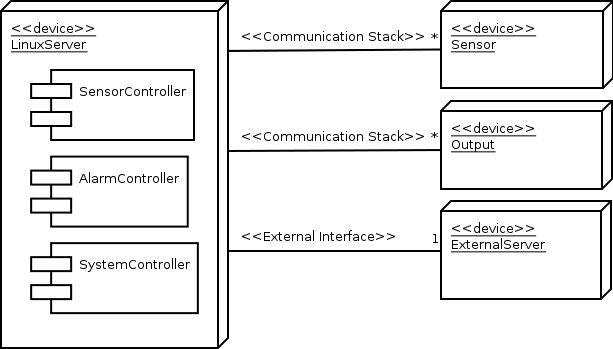
\includegraphics[scale=0.5]{deployment.png}
  \label{fig:subsystem_deployment}
\end{figure}
\floatstyle{boxed}
\restylefloat{figure}

\chapter{System Design} % 10% Zack
\label{ch:system-design}

\section{Hardware/Software Mapping}

The hardware / software mapping of the GARTH system can be viewed at a high
level by examining the subsystem decomposition at the end of Chapter 2. The
external interface and related controllers are software subsystems that are
mapped onto the Linux server. These software components interact directly with
the communications stack implemented by the server. The hardware that is mapped
to the communications stack include the sensors and the inputs and outputs of
the system (such as control panels, alarms, speakers, etc). This hardware maps
specifcally to the hardware interface of the communications stack which
includes all wireless and RF protocol used by the system. The communications
stack also includes the event protocol and communications protocol, which
handle events that are trigged by the hardware. Finally, the external interface
to the system is the software interface of the Linux server which will allow a
user with admin privileges to configure or manipulate the system.

\section{Data Resource Management}
%TODO mentioned proprietary software that should be fleshed out in this SDD

The two main components to GARTH's data resource management are the local
storage hardware and the remote server. The local storage component is
contained within the home and consists of a Linux server that will be stored in
a secure location. The Linux server is a desktop computer with four 2 tera byte
hard drives arranged in a modified RAID array with a parity disk for
redundancy. In this case, if a hard drive should fail the system will continue
to run as expected until a replacement hard drive gets installed. The server
will use proprietary software  to create text files that log system events as
well as store video that is captured by the cameras situated within and outside
the home.
 
The remote server is back-up storage that is located offsite at GARTH
headquarters. It is merely a remote backup of system logs and important video
data that should be saved for future reference. This includes any log-files or
video that was recorded by the system during a critical security violation. This
synchronization will be accomplished by using \textbf{rsync} network protocol
installed on both the local and remote server. The data that is backed up
remotely will be stored in a SQL database such that storing and querying
important data can be accomplished easily.

\section{Access Control and Security}

All access control data will be stored in the local storage database and will be
organized in an access array. The access control array will store user
information, IDs, passwords and priviliges.  This data will be encrypted using
the SHA1 hash algorithm to ensure that this data will be irrelevent to anyone
who accesses it unrightfully. This array can be accessed at any time by the
system to allow necessary access to a user. 

\begin{table}[h]
    \caption{Example of a GARTH access array}
    \label{access_array}
    \centering
    \begin{tabular}{| l | l | l | l | l | l |}
    \hline
    \textbf{Entry ID \#}&\textbf{User ID String}&\textbf{Username}&
    \textbf{Password}&\textbf{NFC ID}&\textbf{Privilege Level} \\ \hline
    1&Daryl Simpson&d\_simpson22&\$taRfi\$h&darylBB&Administrator \\ \hline
    2&Megan Simpson&msimpson&Portia&meganBold&Regular User \\ \hline
    3&Charlotte Simpson&charlotte11&Barbie11&charPod&Restricted \\
    \hline
    \end{tabular}
\end{table}

The array contains relevant information for each person who will be using the
system. The array contains a username and password for each user, in case
they need to log-in through the console's interface to change settings. Certain
settings will only be able to get changed by users with administator access.
The NFC ID field stores the device name of the NFC device the user chose to arm
or disarm the security system.

The access array is useful for determining who can gain access to the system,
however the privileges of each user will be tied separately to their respective
entry in a access control matrix. A standard access control matrix will be
employed by GARTH to solve this problem and can be seen in the table below.

\begin{table}[h]
    \caption{GARTH access control matrix}
    \label{access_control}
    \centering
    \begin{tabular}{| l | l | l | l |}
    \hline
    &\textbf{User Control}&\textbf{Data Control}&\textbf{Security Actions} \\ \hline
    \multirow{4}{*}{\textbf{Administrator}}&
    \textless\textless create\textgreater\textgreater&dumpLogs()&stopAlarms() \\
    &createUser()&searchLogs()&armSystem() \\ 
    &editUser()&viewLogs()&disarmSystem() \\
    &viewUsers()&& \\ \hline
    \multirow{2}{*}{\textbf{Regular User}}&viewUsers()&viewLogs()&armSystem() \\
    &&&disarmSystem() \\ \hline
    \multirow{2}{*}{\textbf{Restricted}}&&&armSystem() \\
    &&&disarmSystem() \\
    \hline
    \end{tabular}
\end{table}

\section{Global Software Control}

Requests are initiated by different inputs throughout the home. Most notable
would be the sensor network that generate event requests depending on the
system's armed state. For example, a window that gets opened while the security
system is armed would trigger an alarm event. Minor events are processed in a
sequential order using a very basic FIFO protocol (no concurrency). However,
events of a critical nature such as a home break-in while the system is armed
will suspend running events and get processed immediately. If more than one
critical event occurs at once, they are queued and handled sequentially while
any current suspended minor events remain suspended. This level of scheduling
will be achieved by using interrupt handling routines for the sensors that
correspond to these events and using global priority queues.Critical events
will be designed such that they are handled quickly and efficiently in order to
avoid circumstances where critical events remained queued for long periods of
time.

\section{Boundary Conditions}

A system administrator is capable of issuing requests for a server reboot,
shutdown, or start-up if the server is powered down. The entire system relies
on the power status of the server, and as such the user can issue these
commands from the server itself (by using its interface) or from any other
control interface in the home.

When the administrator starts the server, the controllers and sensors get
initialized in parallel. Each controller has its own separate initialization
method which starts each process in its reset state. Its own initialization
procedure takes over from here assuming initial conditions of all of its
parameters. These initalization patterns are included in the use case diagram
below as the configuration procedures that extends the initialization
procedures of each controller. The sensor initialization is a more basic
procedure, as the sensors become activated and the system polls their status by
attempting communication between them and the sensor controller. If sensor
communication fails then a sensor error occurs and the system enters a minor
alarm state.

When the administrator shuts down the server, a system snapshot is taken by the
controllers to save the state of all of the subsystems and sensors. This data
is stored in the logs on the server, ready for when the system is started up
again. Once the snapshot is complete and the data has been stored, the power
down scheme begins which first shuts down the sensors, followed by the
controller interfaces, and then finally the server.

A server reboot simply utilizes both of these patterns in order. First a system
shutdown is initiated, followed by a start-up immediately after.

\floatstyle{plain}
\restylefloat{figure}
\begin{figure}[hp]
    \centering
        \caption{Boundary Conditions Use Case Diagram}
        \scriptsize
        \setlength{\unitlength}{2.0em}
        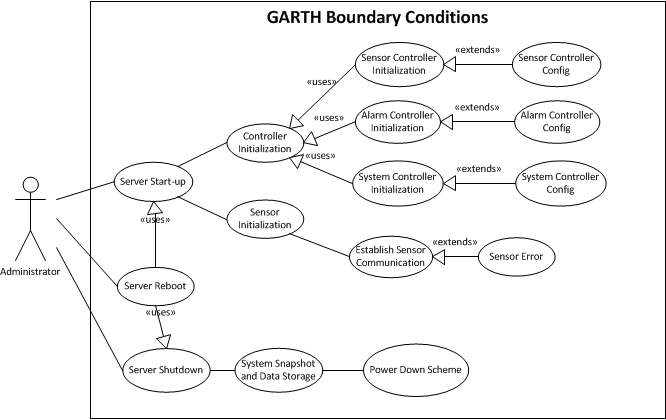
\includegraphics{boundary_conditions.png}
        \normalsize
    \label{fig:boundary_conditions}
\end{figure}
\floatstyle{boxed}
\restylefloat{figure}

\chapter{Interfaces} % 10% - Casey
\label{ch:interfaces}

\section{External System Interfaces}

All interaction with external interfaces is handled by the
SystemController component. This behaviour was chosen to reduce
implementation complexity; if only the SystemController requires
access to external interfaces, then no other Controller will have to
depend on the External Interface subsystem.  This reduces both
compile-time and run-time dependency. A class diagram of the external
interfaces that GARTH uses can be found in
Figure~\ref{fig:external_interfaces}.

\floatstyle{plain}
\restylefloat{figure}
\begin{figure}[hp]
    \centering
        \caption{External System Interfaces}
        \scriptsize
        \setlength{\unitlength}{2.0em}
        \includegraphics{external_interfaces1.mps}
        \normalsize
    \label{fig:external_interfaces}
\end{figure}
\floatstyle{boxed}
\restylefloat{figure}

As shown in the diagram above, there are four main external activites
that can be performed: logging events, initiating a backup, initiating
a remote administration session, and handling external alarms. These
activities can all be performed through the external interface
provided by the external web server.

\section{Internal Subsystem Interfaces}



\chapter{Object Design} % 30% Ben (and Casey?)
\label{ch:object-design}

% For communications Protocol: json-rpc.org/wiki/specification

\section{Design Patterns}

% Describe all design patterns used to reduce complexity and increase re-use in
% the system. Explain how they were applied to specifci components and the
% rationale for them.

Several design patterns have been used in this system. The first is the
singleton design pattern. It was applied to the controllers and the event
manager to ensure that only a single instance of each is made. It also provides
an interface for multithreading support as each instance can be placed on a
separate thread. It also ensures that at most only one controller of each type
is ever handling events during program execution.

A fa\c{c}ade design pattern was used in conjunction with the communications
stack. To reduce the complexity of the interface, a single simpler interface
was provided to handle all of the communication of events to and from the
sensors and other input and output devices.

Creation of events by the \texttt{EventManager} is facilitated by a factory
method pattern. It accepts the strings of arguments and parameters from the RPC
response and translates it into the appropriate event object instance. This
enables new event types and sensors to be added to the system without having to
modify the \texttt{EventManager} class.

The mediator pattern is used for communication between the controllers,
sensors, and other interfaces. The \texttt{EventManager} is the mediator and
mediation is done through the passing of events between subsystems. So as a
result, a class simply has to send an event to the manager and the manager will
send the event off to the appropriate receivers based on the subscription
listing.

\section{Algorithms}

\section{Packages}
The system can be divided into several packages. To increase the brevity of the
diagrams, only one overall package diagram of the system is shown in
Figure~\ref{fig:package_diagram} as a lot of the classes use many of the same
packages. The packages will be broken down into classes with similar to what
the package name is. For the packages that comprise of multiple inherited
subclasses, the inherited classes will have names that better represent their
intended purpose.

\floatstyle{plain}
\restylefloat{figure}
\begin{figure}
    \caption{Package Diagram}
    \label{fig:package_diagram}
    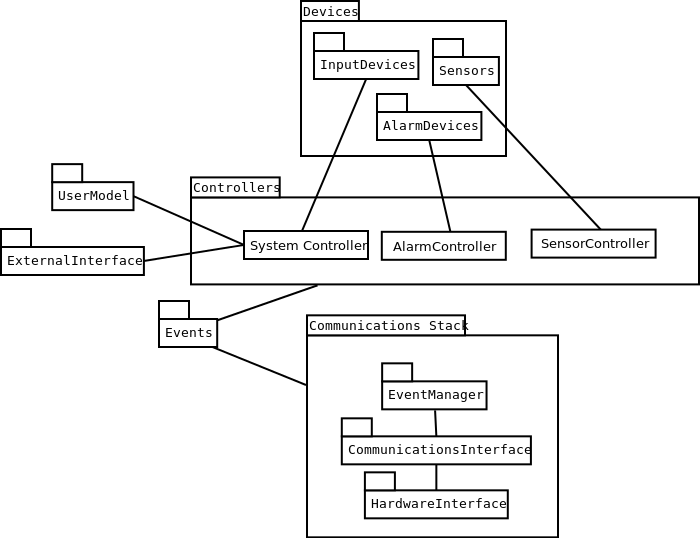
\includegraphics[scale=0.5]{package_diagram.png}
\end{figure}

\section{Object and Interface Design}
A refined class level diagram has been provided for the majority of the
subsystems. For each subsystem, a separate class diagram was generated to keep
things simple and to avoid confusion due to hard to read diagrams. Some
subsystems are provided with other systems due to overlap and to reduce the
number of redundent diagrams.

Each of the controllers are broken up into their own subsystem and are
instantated as singletons. Each controller is derived from the same super class
that provides the abstract method for handling events and the
implementation for subscribing to events with the event manager.

The class diagram for the first controller, the \texttt{SensorController}, and
the sensors are shown in Figure~\ref{fig:sensor_controller_class_diagram}. This
diagram also describes the \texttt{EventType} enumeration which is omitted from
the other diagrams for brevity The \texttt{SensorController} aggregates a list
of sensors, which is fetched from the \texttt{EventManager}. This controller can
explictely poll sensors, handle the sensor input data, and check the sensor
statuses. It sends events to the other controllers through the event manager
after deciding how an event should be handled. 

The sensor subsystem along with the associated sensor events are also described
in Figure~\ref{fig:sensor_controller_class_diagram}. The methods that can be
called on each of the sensors are outlined as well as the associated events that
will be eventually passed back to the controllers. Each sensor event has a
sensor ID number associated with it as well as a specific door or window ID
if it is from a door or a window sensor.

The second controller, the \texttt{SystemController}, is described in the class
diagram in Figure~\ref{fig:system_controller_class_diagram}. It contains all
the methods required with handling inputs from the \texttt{KeypadInputDevice}
and \texttt{NFCReaderInputDevice}. The definition of the class for
\texttt{InputEvent} is included. System state is set and stored within this
controller based on the inputs. Events are recieved from the event manager and
the other controllers which are then sent to the external server and to the
controllers if it is deemed appropriate. This controller also maintains a list
of the user models which is uses to check for authorization rights to see what
the user can do in terms of security actions.

Figure~\ref{fig:alarm_controller_class_diagram} provides the class diagram for
the \texttt{AlarmController} as well as the structure of the
\texttt{AlarmDevice}. This controller handles the operation of the alarm output
devices and the appropriate action for each alarm severity level. There are
several different \texttt{AlarmDevices} that are used for different levels of
alarm severity and alarm causes. An interface is provided to be able to send
external alarms through an HTTP based web interface.

The communications stack class diagram is found in
Figure~\ref{fig:communications_stack_class_diagram}. It represents the entire
communications stack as a summation of three parts, the \texttt{EventManager},
the \texttt{CommunicationsInterface}, and the \texttt{HardwareInterface}. The
\texttt{EventManager} is the layer accessible to the controllers. It provides
methods to access the layers beneath it indirectly. It maintains two event
queues, one for the input events from the sensors and one priority queue for
the alarm events. It takes a hash map of strings that map to events and
converts it into events to pass to the controllers based on the event
subscription list. Events are handled in a FIFO queue until it is empty and
once it is empty, occasionaly checked on a timer to ensure that new events are
looked after promptly.

The next layer, the \texttt{CommunicationsInterface} deals with the encoding
and decoding of the remote process communication with the sensors. Sensors are
polled or status checked based on sensor ID which is used to get sensor data
from the next layer down so that the RPC can be encoded properly. This class
takes the response string from the \texttt{HardwareInterface} and converts it
into a HashMap with the arguments and parameters from the RPC response.

Hardware is communicated to through the \texttt{HardwareInterface}. It also
stores a list of all the sensors, alarm devices, and input devices. Encoded RPC
strings can be sent from the \texttt{CommuncationsInterface} through this layer
to either the sensors or alarm devices. Any device can send a response as an
encoded RPC string even if it was not requested by a controller. This provides
a means of event driven communication between the sensors and the controllers
without relying on tight polling from the \texttt{SensorController}.
\begin{landscape} 
\floatstyle{plain}
\restylefloat{figure}
\begin{figure}[p]
    \caption{\texttt{SensorController} and \texttt{Sensor} Class Diagram}
    \label{fig:sensor_controller_class_diagram}
    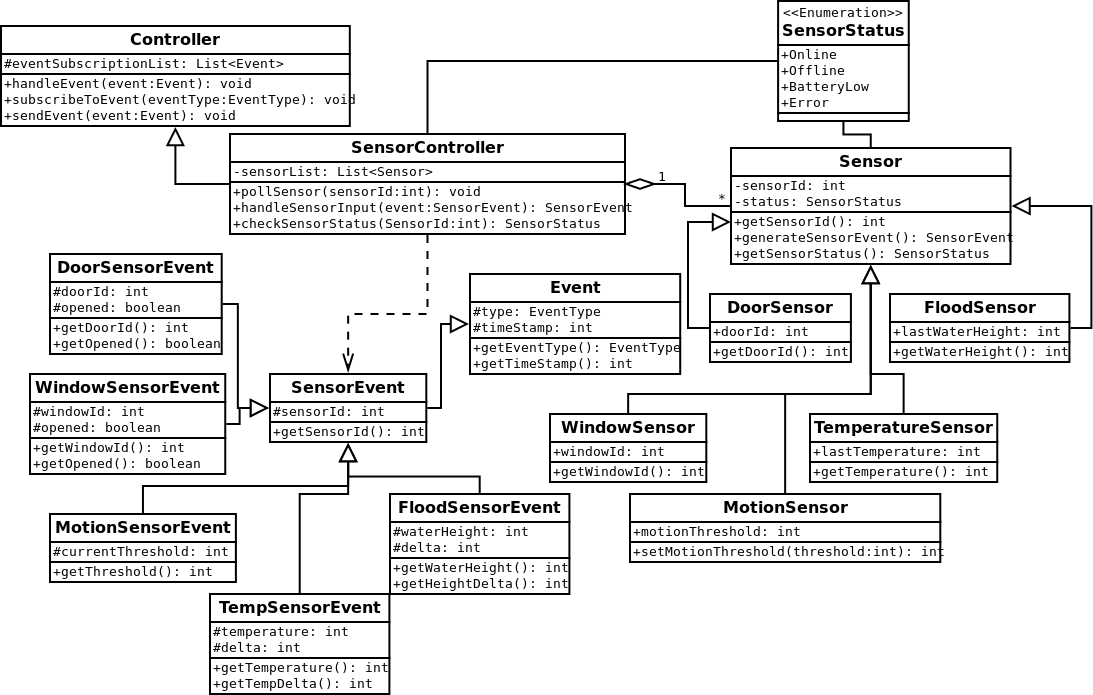
\includegraphics[scale=0.5]{sensor_controller_class_diagram.png}
\end{figure}
\end{landscape} 

\begin{landscape} 
\floatstyle{plain}
\restylefloat{figure}
\begin{figure}[p]
    \caption{\texttt{SystemController} Class Diagram}
    \label{fig:system_controller_class_diagram}
    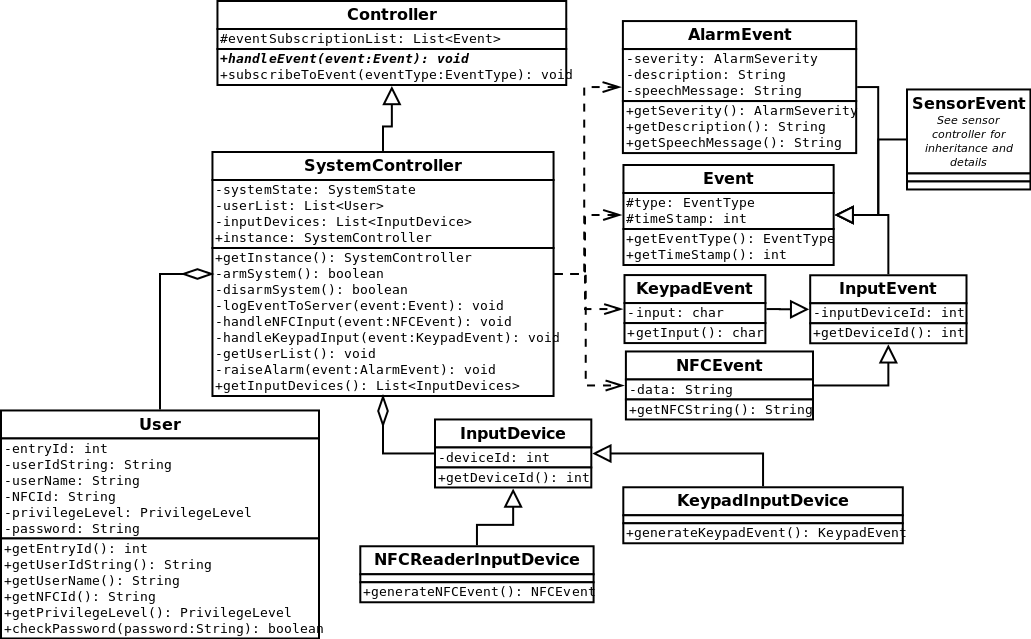
\includegraphics[scale=0.5]{system_controller_class_diagram.png}
\end{figure}
\end{landscape} 

\begin{landscape}
\floatstyle{plain}
\restylefloat{figure}
\begin{figure}[p]
    \caption{\texttt{AlarmController} Class Diagram}
    \label{fig:alarm_controller_class_diagram}
    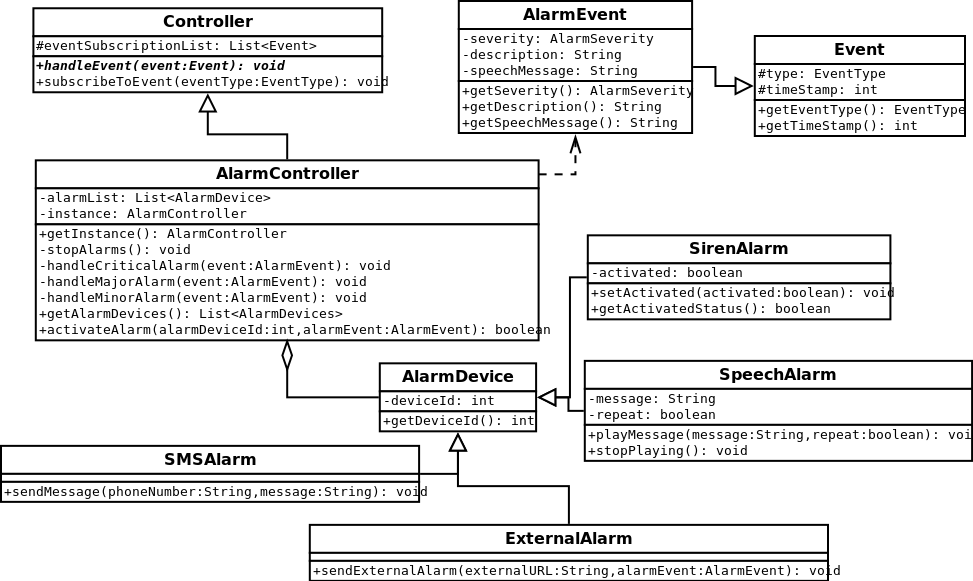
\includegraphics[scale=0.5]{alarm_controller_class_diagram.png}
\end{figure}
\end{landscape}

%\begin{landscape}
\floatstyle{plain}
\restylefloat{figure}
\begin{figure}[p]
  \centering
  \caption{Communications Stack Class Diagram}
  \label{fig:communications_stack_class_diagram}
  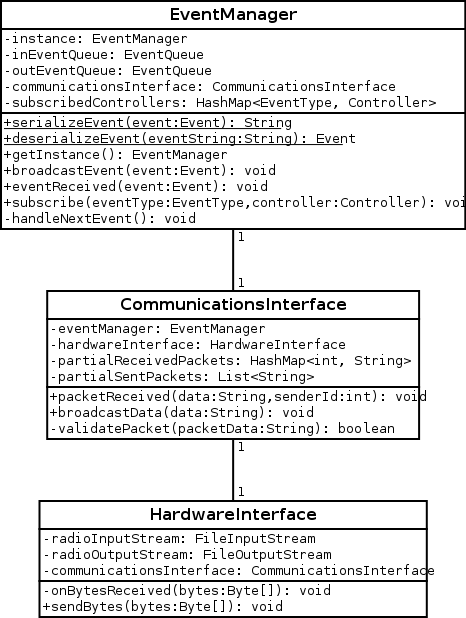
\includegraphics[scale=0.5]{communication_stack_class_diagram}
\end{figure}
%\end{landscape}

\section{Dynamic Design Model}

\chapter{Design Evaluation} % 10% Zack
\label{ch:design-evaluation}

\section{Design Trade-offs}

During design of the GARTH system, many key decisions were made that affected
the overall performance, functionality, and cost of the system. These are key
aspects that were considered in the design, but some decisions had to be
weighed in order to maintain balance in the design. For example, performance
optimization was a goal to make sure that the system was robust and adequately
reactive to certain events, but resulted in more expensive hardware and
software implementation. Also, the system was designed such that it was
functionally robust but much attention needed to be paid to functionality to
make sure that it was still intuitive and easy to use. Certain other decisions
like whether to use store-bought implementation vs. proprietary hardware and
software factored into this discussion as well.

The GARTH home system is designed to be robust in many areas, one in particular
is its performance. Not many shortcuts were taken in ensuring that the system
will be able to react to security events quickly and seamlessly. This is ideal
for a security system of this magnitude, but it introduced higher engineering
costs. For example, high-speed wireless protocols were included in the design
to ensure quick and reliable communication of the system throughout the home.
This is more expensive than using a wired network or even RF wireless protocol
but ultimately results in a more responsive system. Since GARTH is a total home
security solution, performance was regarded with slightly higher priority than
cost optimization due to the target demographic of the system which is
typically high income households.

Much attention was paid to the usability of the system. The user interfaces
will be implented in such a way that they are inherently intuitive to a new
client that has purchased and installed the system for the first time. The idea
behind this philiosophy is that in order to use the system the client should
not have to read extensive documentation in order to learn how to configure,
manage, arm or disarm any features of the system. This implementation is very
suitable for the user, but requires that extra attention is paid to making sure
the system is still functionally adequate. Therefore, another trade-off that
was made was enforcing strong usability and functionality in the same vein. As
a result, the software design cost of the system was slightly increased as more
support architecture was required to make up for how simple the system appears
to the user.

When choosing hardware for the GARTH home system, a lot of store-bought
equipment was chosen over implementing proprietary solutions. Sensors, cameras,
microcontrollers, and servers were selected from buyable solutions for
simplicity and availability. For example, the main server that controls the
GARTH system and stores user data is a Linux server built from store-bought
parts.  This makes the system very easily supportable as there is currently a
lot of documentation and manufacture support for these parts. Open source
software like the Linux operating system will be used where available to reduce
cost.

\section{Re-use}

Through inheritance and delegation, many classes were able to be re-used in the
object model of the system. This proved to be very useful as much of the design
was simplified due to the re-use of these objects. Within the GARTH system,
events and how they are handled are crucial to the functionality of the system.
Since the system can respond to many different situations within the home,
GARTH needed many different event classes to be added to the object diagram.
Through inheritance however, using the event class, the design was very simple
to extrapolate to the many different event classes needed within the object
model. For example, within the sensor controller and sensor class model the
door sensor event model, window sensor event model, and motion sensor event
model all inherit from the sensor event class, which inherits from the overall
event class. This will make it very easy for the software designers of GARTH to
extrapolate if needed when more event classes are designed. There is also a
general sensor class that defines overall sensor behaviour throughout the home.
Many different sensors in the GARTH system inherit from this class to re-use
common parameters while still providing unique behaviour over the different
kinds of sensors. The sensor controller model also inherits from the controller
class.

Within the system controller class diagram, an input device class was defined
that allowed the different input devices that the users interact with to
inherit from it. The keypad input device as well as the NFC reader devices
inherit from this class. The system controller object model also includes new
events that re-use the event model mentioned previously. Also, the system
controller class itself inherits from the controller model.

Much like the other controller class models, the alarm controller class
inherits from the controller class. Also its alarm event class inherits from
the overall event class much like the other controller classes. This object
model varies from the others in that it introduces the alarm device class. This
class defines the different alarms that are triggered by the system. The
classes SMS alarm, speech alarm, external alarm, and siren alarm all inherit
from this class.

\section{Optimizations}

One of the optimizations that was made from the last iteration of the GARTH
design to now is how events propagate through the system and communicate with
the devices that deal with said events. Previously, every device was able to
talk to each other to pass event information through the system to be handled by
the server. This resulted in a much more complicated object model as well as
more complicated hardware. Now, the communications stack has a specific event
protocol and framework built in in order to handle all of the events. When an 
event occurs, it gets passed through this framework and is dealt with by the
server directly which is much more efficient.

Another change that was made was to the controller class objects. The controllers
have been made into singleton objects, which is useful as there is only one
instantiation of each of the controller types. The only complication this produces
is that these singleton classes introduce global state into the design, which
is fortunately mitigated by the fact that we have boundary control to initialize
and configure these controller classes individually. 

Lastly, a user model class was added to the object diagram in order to help
define the actors using the system. It became apparent that a user model would
need to be added to the object model once the access control portion of the 
system was fleshed out. Paramaters included in the access array such as user
name strings, password hashes, and privilege levels needed to be stored in
objects for simplicity, so this functionality was added in this iteration of the
design.

\section{Extensibility}

The GARTH system was designed such that it is easily extendable, by making good
use of inheritance and design patterns that encourage extensibility. Since many
of our controller class models make use of re-use in class objects such as
events, alarms, and sensors, if anything of this type needs to be added to the
system it is very simple to do since they can inherit from the general class
models that already exist. For example, if a server alarm were added to the
system in the event that the server is in risk of being compromised, this
situation could easily be added to the object model by creating a new sensor
model, event model, and alarm model that correspond to it.

Extensibility in design patterns are also used, as the communication stack
implements the fa\c{c}ade design pattern when interfacing with the rest of the
system with regards to communication. If a new sensor, event, or alarm needs to
be added to the system, this design pattern makes it very easy to expand the
interfaces to interact with the new components of the system.

\chapter{Operating Environment} % 10% Ben 
\label{ch:operating-environment}

\section{Development Platform}
%In general terms, describe the anticipated platform on which this system will
%be developed, including the implementation language, major libraries and
%network protocols utilized, and special language or OS or middleware features
%used, such as remote procedure calls, a built-in event handling model, user
%interface library, etc.

% TODO :: talk about any special language, OS, or middleware features used

Development will be done under a Linux environment as it closely matches the
intended runtime platform for the server. It also has support for all of the
required tools and libraries that are going to be used. 

Implementation language depends on the particular subsystem of the application.
The controllers will be implemented in Python for quick development and ease of 
maintenance. The sensors will need to be programmed in C for efficiency and
simplicity. Although this is not a purely Object Oriented language, using C++
would be ineffective as it results in more overhead that is to be avoided in a
real time system such as a sensor. The mobile applications will be written in
Objective-C for the iOS application and in Java for the Android version as
required by the platforms.

Several network protocols will be used. The Zigbee protocol, IEEE
802.15.4, will be used for the hardware level communication between
sensor nodes and the base station. External interfaces will use TCP/IP
through HTTP requests for retrieving or modifying data.

On the iOS platform, the user interface will be constructed with the Quartz and
UIKit. These libraries provide common user interface elements such as labels,
buttons, and more. For HTTP requests, the AFNetworking library will be used as
it simplifies the handling network requests and all of the boilerplate
associated with it. On Android, the standard libraries will be used as they are
sufficient and no third party libraries exist that are provide better
functionality then the stock ones.


% Reference this: afnetworking.org/Documentation

\section{Runtime Platform}
The platform is divided into two major types of components, controllers and
sensors. Both types have different requirements for operating systems and
hardware. Middleware is required to interface between the two subsystems as
well. 

The controllers will all operate on a single server as seperate processes. The
server will be a Linux based server orientated distribution such as CentOS or
Debian. The server will be housed locally within the house. The hardware needs
to be powerful, yet energy efficient and compact. No dependance on exact
hardware is required. Some recommended specifications are outlined in
Table~\ref{server_hardware}.

Each sensor will have its own independent hardware and operating system due to
the independent nature of these devices. Each will have an Atmel AVR ATMega
microcontroller for reading sensor data and communicating through the Zigbee.
The tinyOS operating system can be used to quicken development time and the
protocols for communication with the Zigbee. The tinyOS will also simplify
setting up the mesh network as several modules are provided for this.

Some middleware is required to interface the sensors and the controllers
through a Zigbee and microcontroller connected via USB to the server. A simple
hardware interface is required to allow for two-way communication between the
controllers and the sensors.

\begin{table}[h]
    \caption{Recommended Server Hardware}
    \label{server_hardware}
    \centering
    \begin{tabular}{| c | p{5cm} |}
    \hline
    Processor & AMD Athlon II X3 445 \\ \hline
    Motherboard & ASUS M5A78L-M LX PLUS AMD 760G Motherboard - Micro ATX,
    AMD 760G Chipset, 1866MHz DD3 (O.C.), SATA 3.0 Gb/s, RAID, Gigabit LAN \\
    \hline
    Case &  XION XON-810P-Red Micro ATX/ITX with 450W PSU \\ \hline
    Memory & Corsair Value Select PC10600 RAM - 2GB, DDR3, 1333Mhz \\ \hline
    Hard Drives & Western Digital Caviar Green - 2 TB x 4 \\
    \hline
    \end{tabular}
\end{table}


\section{Process Model}
The system as a whole is distributed system, with subsystems consisting of
concurrent processes or single threaded microcontrollers. The sensor network is
one distributed subsystem that consists of many single process
microcontrollers. 

The controllers and the communciation stack located on the server are
concurrent threads which can communicate freely using inter-thread techniques.
Communication is done through the \texttt{EventManager} thread as seen in
Figure~\ref{fig:communications_stack_class_diagram}, the communications stack
class diagram. This enables easy synchronization through events queues where
the events are the messages of a traditional message queue.

\section{Synchronization}
%Describe the method of coordination and synchronization between software
%tasks, such as semaphores or message queues.

% TODO :: More
Coordination and synchronization between software is done through message
queues. More specifically, the event objects are passed between interfaces and
are handled as the messages in the event queues. These event queues will
have different priority levels as some events are more critical then others in
terms of time sensitivity. 

Synchronization between the hardware interface and the sensors will be done
thorugh the ZigBee protocol to ensure that the complete message has been
received before trying to parse the information. This protocol defines error
conditions, 

\section{Fault Handling}
Errors will be handled on a case by case basis as some errors will not affect
day to day operation of the system. Minor errors such as a temperature misread
or missing data from one of the passively read sensors can be ignored as long
as it is a transient event. Major errors such as a missing sensor or low
battery levels on a sensor will need to be handled. Critical errors such as a
hardware failure in the base station or server will require special care.

Minor errors can be ignored for the most part. These represent one time sensor
misreads, missing data, and other faults that do not affect any long term
operation of the system. These minor faults still need to be accounted for as
multiple occurances of this type will imply an issue with the sensor or
communication interface. When a minor error is detected, the error needs to be
logged but no further action is required.

Major errors will require system action and possibly user action to correct.
Major faults include missing sensors, low battery levels, and other issues that
will affect the short-term and long-term operation of the system. These faults
need to be accounted for and handled appropriately. In some cases, the user
will need to alerted with information on how to take the appropriate actions.
For example, if a sensor has low battery levels then the user will need to
replace or recharge the battery to ensure proper and continuous operation.

The final error criticality level is critical faults. Complete hardware or
software failures of the server can be considered critical faults. If the fault
is easily recoverable, such as a brown out causing a power flicker at the
house, then the components effected need to restart as quickly as possible to
ensure proper and consistent operation. For other faults such as hardware
failure in the base station or the server, then the user will need to take
appropriate action to fix the malfunctioning hardware.

All of these, if it is required, can be handled as \texttt{AlarmEvents} with
the appropriate alarm severity. Some events, like the minor data misreads will
not need to be report. This will ensure that all events of significant meaning
will be forwarded to the appropriate controller and the users notified of the
occurance of an error.

\end{document}
